\chapter{Algebraic Geometry}\label{chapter:alggeom}

    References for this chapter are~\citet{gathmann_algebraic_2019,mumford_red_1999,vakil_foundations_2023,vakil_math_2025,hartshorne_algebraic_1977}. For the basics on ring theory, ideals and algebraic dependence, see \namecrefs{section:ring}~\ref{section:ring} and~\ref{section:algebraic_numbers}, and for some background on ringed spaces, see \cref{section:ringed_spaces}. The section on tropical geometry is mainly based on~\citet{maclagan_aarms_2008}. In order to not confuse the letters $k$ and $K$, often used for fields, with various indices and dimensions, fields will be denoted by the symbol $\mathfrak{K}$ in this chapter. Moreover, the base field $\mathfrak{K}$ will also be assumed to be algebraically closed (unless noted otherwise).

    \minitoc

\section{Varieties}\label{section:varieties}

    For notational simplicity and to differentiate between $\mathfrak{K}^n$ as a vector space and as a set, the notion of an affine space is introduced.
    \newdef{Affine space}{\index{affine!space}
        $\mathbb{A}^n$ is defined as the underlying set of the vector space $\mathfrak{K}^n$:
        \begin{gather}
            \mathbb{A}^n := \bigl\{(a_1,\ldots,a_n)\in \mathfrak{K}^n\bigr\}.
        \end{gather}
    }

    \newdef{Algebraic set}{\index{algebraic!set}\index{irreducible!algebraic set}\index{variety}\label{alggeom:variety}
        Consider a finite set of polynomials in $\mathfrak{K}[x_1,\ldots,x_n]$. It is not hard to show that the zero locus of these polynomials depends only on the ideal spanned by them and, hence, one can define the algebraic set associated to an ideal $I\subseteq \mathfrak{K}[x_1,\ldots,x_N]$ to be
        \begin{gather}
            V(I) := \bigl\{(a_1,\ldots,a_n)\in\mathbb{A}^n\bigm\vert\forall f\in I:f(a_1,\ldots,a_k)=0\bigr\}\,.
        \end{gather}
        A set $S\in\mathbb{A}^n$ is said to be an \textbf{(affine)} algebraic set if there exists an ideal $I$ such that $S=V(I)$. An algebraic set $S\in\mathbb{A}^n$ is said to be \textbf{irreducible} if it is not the union of two strictly smaller algebraic sets. Irreducible algebraic sets are also called \textbf{affine varieties}.
    }
    \sremark{Some authors, such as~\citet{gathmann_algebraic_2019}, make no distinction between general algebraic sets and affine varieties.}

    \begin{property}\index{Hilbert!basis theorem}
        By Hilbert's basis theorem~\ref{algebra:hilbert_basis_theorem}, any algebraic set can be expressed as the zero locus of a finite number of polynomials.
    \end{property}

    Given an algebraic set $S$, the set $I(S)$ is defined as the ideal of polynomials that vanish on $S$. The following theorem gives an important relation between algebraic sets and ideals.
    \begin{theorem}[Hilbert's Nullstellensatz]\index{Hilbert!Nullstellensatz}\index{Nullstellensatz|seealso{Hilbert}}
        Let $J$ be an ideal in $\mathfrak{K}[x_1,\ldots,x_n]$ and let $\sqrt{J}$ denote its radical (\cref{algebra:radical}).
        \begin{gather}
            I\bigl(V(J)\bigr) = \sqrt{J}
        \end{gather}
    \end{theorem}
    Similar to the case of the weak Nullstellensatz, one obtains the following result.
    \begin{result}
        There exists a bijection between the algebraic subsets of $\mathbb{A}^n$ and the radical ideals in $\mathfrak{K}[x_1,\ldots,x_n]$. The irreducible algebraic sets correspond to the prime ideals by the Lasker--Noether decomposition theorem~\ref{algebra:lasker_noether}.
    \end{result}

    \newdef{Rational point}{\index{rational!point}\label{alggeom:rational_point}
        Let $V\subseteq\mathfrak{K}^n$ be an affine variety and let $\{f_i\}_{i\leq r}$ be a set of generating polynomials. The rational points $V(\mathfrak{K})$ are exactly the solutions of the system of equations
        \begin{gather}
            \begin{cases}
                &f_1(x_1,\ldots,x_n)=0\\
                &\vdots\\
                &f_r(x_1,\ldots,x_n)=0\,.
            \end{cases}
        \end{gather}
    }

    \newdef{Morphism of varieties}{\index{morphism!of varieties}
        Let $V_1\subset\mathbb{A}^{n_1},V_2\subset\mathbb{A}^{n_2}$ be two affine varieties. A morphism $\varphi:V_1\rightarrow V_2$ is a function that can be expressed in the following way:
        \begin{gather}
            \varphi(x_1,\ldots,x_{n_1}) = \bigl(f_1(x_1,\ldots,x_{n_1}),\ldots,f_{n_2}(x_1,\ldots,x_{n_1})\bigr)\,,
        \end{gather}
        where $f_i\in\mathfrak{K}[x_1,\ldots,x_{n_1}]$ for all $i\leq n_2$.
    }
    A closely related notion is that of rational maps.
    \newdef{Rational map}{\index{rational!map}\index{dominant}\index{bi-!rational|see{rational}}
        Consider two affine varieties $X,Y$. A rational map $f:X\rightarrow Y$ is an equivalence class of pairs $(U,f_U)$, where $U$ is a nonempty open subset and $f_U:U\rightarrow Y$ is a morphism of varieties, under the following relation: $(U,f_U)\sim(V,f_V)$ if and only if $f_U=f_V$ on a nonempty subset of $U\cap V$.

        A rational map is said to be \textbf{dominant} if, for one of its representatives $(U,f)$, the image $f(U)$ is dense. Dominance of rational maps assures that their composition exists and is well-defined. A rational map $f:X\rightarrow Y$ is said to be \textbf{birational} if it is dominant and admits a rational inverse.
    }

    \newdef{Coordinate ring}{\index{coordinate!ring}\index{function!field}\index{rational!function}\label{alggeom:coordinate_ring}
        Consider the polynomial ring $\mathfrak{K}[x_1,\ldots,x_n]$ and let $V$ be an algebraic set in $\mathbb{A}^n$. The coordinate ring (or \textbf{affine ring}) of $V$ is defined as the following quotient:
        \begin{gather}
            \Gamma(V) := \mathfrak{K}[x_1,\ldots,x_n]/I(V)\,.
        \end{gather}
        The elements of this ring are the $\mathfrak{K}$-valued polynomials in the coordinates on $V$.

        If $V$ is irreducible, it follows from the Nullstellensatz that $I(V)$ is a prime ideal and, hence, that $\Gamma(V)$ is an integral domain. This property allows to construct the field of fractions (\cref{algebra:fraction_field}). This field is called the \textbf{function field} of $V$ and is denoted by $\mathfrak{K}(V)$. The elements of $\mathfrak{K}(V)$ are called the \textbf{rational functions} on $V$. It can be shown that the rational functions are exactly the rational maps $V\rightarrow\mathbb{A}^1$.
    }

    It should be noted that every morphism of varieties induces a $\mathfrak{K}$-morphism on the associated affine rings by precomposition. This gives rise to the following property.
    \begin{property}[Finitely generated algebras]\label{alggeom:variety_domain_equivalence}
        $\Gamma$ gives an equivalence between the category of algebraic sets and the category of finitely generated (reduced) $\mathfrak{K}$-algebras. This equivalence passes to an equivalence between the subcategories on affine varieties and integral domains.
    \end{property}

    \newdef{Dimension}{\index{dimension!of variety}\index{Krull!dimension}
        The dimension of an affine variety is given by the \textbf{Krull dimension} of its coordinate ring, i.e.~the maximum length of a chain of prime ideals in $\Gamma(X)$:
        \begin{gather}
            \dim(X) := \sup_{n\in\mathbb{N}}(\exists\,\mathfrak{p}_0\subsetneq\mathfrak{p}_1\subsetneq\cdots\subsetneq\mathfrak{p}_n)\,.
        \end{gather}
        By the Nullstellensatz this is equivalent to the maximum length of chains of irreducible algebraic subsets.

        The \textbf{local dimension} $\dim_p(X)$ of a point $p\in X$ is defined in a similar way, with the start of the chains fixed at $\{p\}$. One then obtains
        \begin{gather}
            \dim(X) = \max_{p\in X}\dim_p(X)\,.
        \end{gather}
    }

\subsection{Topology}

    A topology on an affine variety can be constructed in the following way.
    \newdef{Zariski topology}{\index{Zariski!topology}
        A set in $\mathbb{A}^n$ is deemed closed exactly if it is an algebraic set. A basis for this topology is given by the complements of zero loci
        \begin{gather}
            B_f=\{x\in\mathbb{A}^n\mid f(x)\neq 0\}
        \end{gather}
        for $f\in\mathfrak{K}[x_1,\ldots,x_n]$. This topology turns an affine variety into an irreducible space.

        On an algebraic subset $V\subset\mathbb{A}^n$, one defines the Zariski topology as the induced topology of the one on $\mathbb{A}^n$. A basis for this induced Zariski topology is given by the sets $B_f$ as above, but where $f$ is now an element of $\Gamma(V)$.
    }

    The following property shows that the Zariski topology is very different from the topologies that occur in, for example, analysis.
    \begin{property}[Density]
        Any open subset of an affine variety is dense. Moreover, if $\mathfrak{K}$ is separably closed, the set of rational points $V(\mathfrak{K})$ is dense as well.
    \end{property}

    By dualizing, one can focus on the coordinate rings and construct varieties as a derived notion. In this approach, the main tool is the structure sheaf of a variety and, accordingly, the content of \labelref{chapter:sheaf} on sheaf theory will, from here on, become a prerequisite.
    \newdef{Structure sheaf}{\index{structure!sheaf}\index{regular!function}\label{alggeom:structure_sheaf}
        Consider an affine variety $X$ with its associated coordinate ring $\Gamma(X)$. For any point $x\in X$, one can consider the set of functions $m_x\subset\Gamma(X)$ that vanish at $x$. This is a prime ideal, so one can construct a localization:
        \begin{gather}
            \mathcal{O}_x := \Gamma(X)_{m_x} = \{f/g\mid f,g\in\Gamma(X)\land g(x)\neq0\}\,.
        \end{gather}
        For every open subset $U\subset X$, one can then define the ring of functions on $U$ as follows:
        \begin{gather}
            \mathcal{O}_X(U) := \bigcap_{x\in U}\mathcal{O}_x\,.
        \end{gather}
        $\mathcal{O}_X$ is a sheaf with stalks given by $\mathcal{O}_x$. By \cref{algebra:localization_local_ring}, all stalks $\mathcal{O}_x$ are local rings and, hence, $(X,\mathcal{O}_X)$ is a locally ringed space (\cref{sheaf:locally_ringed_space}). The residue field of these local rings is equal to the base field $\mathfrak{K}$. The elements of $\mathcal{O}_X(U)$ are called the \textbf{regular functions} on $U$.

        This construction can be made more explicit. A map $\varphi:X\rightarrow\mathfrak{K}$ is said to be \textbf{regular} at a point $x\in X$ if there exists an open neighbourhood $U\ni x$ and polynomials $f,g\in\Gamma(X)$ such that $g\neq0$ and $\varphi=f/g$ on $U$. As for continuous functions, the map $\varphi$ is said to be regular on $X$ if it is regular at every point $x\in X$.
    }

    \begin{property}
        Let $f\in\Gamma(X)$ be a function on $X$ and consider the basis set $B_f$, i.e.~the complement of the zero locus of $f$. The structure sheaf assigns localizations to basis sets:
        \begin{gather}
            \mathcal{O}_X(B_f) = \Gamma(X)_f\,.
        \end{gather}
        In particular,
        \begin{gather}
            \Gamma(X,\mathcal{O}_X) = \Gamma(X)\,,
        \end{gather}
        where, on the left-hand side, $\Gamma$ denotes the global sections functor~\ref{sheaf:global_sections_functor}. This property explains the notation $\Gamma(X)$ introduced before.
    \end{property}
    \remark{Both $\mathcal{O}_X(U)$ and $\mathcal{O}_x$ are subrings of the function field $\mathfrak{K}(X)$.}

    \newadef{Affine variety}{\index{variety!affine}
        A topological space $X$ equipped with a sheaf $\mathcal{F}$ of $\mathfrak{K}$-valued functions such that $X$ is isomorphic to an irreducible algebraic set $\Sigma$ and such that $\mathcal{F}$ is isomorphic to the structure sheaf $\mathcal{O}_X$. An open subset of an affine variety is sometimes called a \textbf{quasi-affine variety}.
    }
    Using the notion of a regular function, the definition of a morphism of affine varieties can be restated.
    \newadef{Morphism}{\index{morphism!of varieties}
        A continuous function between affine varieties $f:X\rightarrow Y$ such that precomposition by $f$ preserves regular functions.
    }

    \begin{property}[Identity theorem]\index{identity!theorem}
        If two regular maps coincide on a nonempty open subset, they are equal.
    \end{property}

    \newdef{Generic stalk}{\index{stalk!generic}
        For the construction of the stalk of the structure sheaf over a point $x\in X$, one takes a direct limit over all open sets containing $x$. This way, the local ring $\Gamma(X)_{m_x}$ is obtained. Moreover, this is a subring of the field of fractions $\mathfrak{K}(X)$ of $\Gamma(X)$. Now, using a similar definition, one can recover all of $\mathfrak{K}(X)$.

        Instead of taking a direct limit over the open sets containing a certain point $x\in X$, take a direct limit over all open sets in $X$:
        \begin{gather}
            \mathcal{O}_{\tilde{x}} := \varinjlim_{U\subset X}\mathcal{O}_X(U)\,.
        \end{gather}
        This stalk is called the generic stalk of $X$ and it is isomorphic to $\mathfrak{K}(X)$.
    }

    \newdef{\'Etale morphism over algebraically closed fields}{\index{etale!morphism}\label{alggeom:etale_morphism_variety}
         A morphism $f:X\rightarrow Y$ of affine varieties over an algebraically closed field such that the induced maps $\widehat{\mathcal{O}}_{f(x)}\rightarrow\widehat{\mathcal{O}}_x$ on the completions (\cref{algebra:ring_completion}) of local rings are isomorphisms.
    }

    \begin{property}[Dimension]\index{dimension!of a prevariety}
        The dimension of a variety $X$ over a field $\mathfrak{K}$ is equal to the transcendence degree (\cref{algebra:transcendence_degree}) of its function field $\mathfrak{K}(X)$.
    \end{property}
    \begin{result}
        Let $X$ be a prevariety over an algebraically closed field $\mathfrak{K}$. If $\dim(X)=0$, then $X=\{\ast\}$, since a vanishing transcendence degree implies that the extension is algebraic.
    \end{result}

    \newdef{Pure dimension}{\index{dimension!pure}
        A closed subset $Z\subseteq X$ is said to be of pure dimension or \textbf{equidimensional} of dimension $n\in\mathbb{N}$ if every irreducible component is of dimension $n$.
    }

    \begin{property}[Closed point]
        Closed points of a prevariety correspond to maximal ideals of the coordinate ring.
    \end{property}

    \begin{remark}[Product]\index{product!of varieties}
        Over a general field, the (fibre) product of varieties is not a variety. Over algebraically closed fields, however, this is the case.
    \end{remark}

\subsection{Varieties}

    \newdef{Prevariety}{\index{pre-!variety}
        A connected, locally ringed space that admits a finite cover by affine spaces.
    }

    \begin{remark}
        It can be shown that every prevariety $X$ is irreducible and, hence, the open sets form a direct system. This way, one can define the \textbf{generic stalk} of an arbitrary sheaf $\mathcal{F}$, as in the case of affine varieties. For the structure sheaf $\mathcal{O}_X$, this generic stalk is again called the \textbf{function field} $\mathfrak{K}(X)$. It coincides with the function field of every open affine subset of $X$.
    \end{remark}

    \begin{construct}[Gluing]\label{alggeom:gluing}
        Consider two prevarieties $X,Y$ together with an isomorphism $f:U\cong W$ between open subsets $U\subset X,V\subset Y$. The prevarieties can be glued together along $f$ as follows. First, build the attaching space (\cref{topology:attaching_space}) $U\cup_fY$ with its canonical topology. Then, define the regular functions on a subset to be those that come from regular functions on (subsets of) $X$ and $Y$.
    \end{construct}

    \newdef{Variety\footnotemark}{\index{variety}\label{alggeom:abstract_variety}
        \footnotetext{Sometimes also called a \textbf{separated variety}, in which case prevarieties are called varieties.}
        A prevariety $X$ for which the diagonal $\Delta_X$ is closed in $X\times X$. It should be noted that every affine variety is a variety.
    }
    \begin{remark}
        The motivation for this definition is \cref{topology:hausdorff}. In general topology it is well-known that a lot of pathological spaces can be excluded by restricting to Hausdorff spaces, i.e.~spaces where distinct points admit disjoint neighbourhoods. Because open subsets of irreducible spaces have nonempty intersections, this property is sadly enough not very useful in the study of varieties. However, the equivalent definition using closedness of the diagonal remains useful if one does not consider the product topology on $X\times X$, but instead uses the `gluing'-topology from \cref{alggeom:gluing} above.
    \end{remark}

    The following two closure properties are very important.
    \begin{property}\label{alggeom:closed_graph}
        Consider a prevariety morphism $f:X\rightarrow Y$, where $Y$ is a variety. The graph of $f$ is closed in $X\times Y$.
    \end{property}
    \begin{property}
        Consider two prevariety morphisms $f,g:X\rightarrow Y$ where $Y$ is a variety. The set on which $f$ and $g$ coincide is closed in $X$.
    \end{property}

\subsection{Projective varieties}

    \newdef{Projective space}{\index{projective!space}\label{alggeom:projective_space}
        Consider the vector space $\mathfrak{K}^n$. The projective space $\mathbb{P}_{n-1}(\mathfrak{K})$ or $\mathfrak{K}\mathbb{P}^{n-1}$ is defined as the quotient of $\mathfrak{K}^n$ under the following equivalence relation:
        \begin{gather}
            (x_1,\ldots,x_n)\sim(y_1,\ldots,y_n)\iff\exists\lambda\in \mathfrak{K}^\times:\forall i\leq n:x_i=\lambda y_i\,.
        \end{gather}
        The equivalence class of a vector $(x_1,\ldots,x_n)$ is denoted by $[x_1:\cdots:x_n]$. Because the numbers characterizing an equivalence class are only determined up to a common factor, the coordinates $x_1,\ldots,x_n$ are called \textbf{homogeneous coordinates}.
    }

    Consider the subset
    \begin{gather}
        \mathfrak{K}_{\text{hom}}[x_0,\ldots,x_n]\subset \mathfrak{K}[x_0,\ldots,x_n]
    \end{gather}
    consisting of all homogeneous polynomials. The definition of projective space implies that
    \begin{gather}
        \forall f\in \mathfrak{K}_{\text{hom}}[x_0,\ldots,x_n]:f(\lambda x_0,\ldots,\lambda x_n) = 0\iff f(x_0,\ldots,x_n) = 0
    \end{gather}
    and, hence, that the zero loci of homogeneous polynomials are well-defined subsets of the projective space $\mathbb{P}_n(\mathfrak{K})$.
    \newdef{Projective algebraic set}{\index{algebraic!set}\index{Zariski!topology}
        As in the case of affine algebraic sets one can define two operations. Let $I$ be a homogeneous ideal, i.e.~an ideal in $\mathfrak{K}[x_0,\ldots,x_n]$ that is generated by homogeneous polynomials. The projective algebraic set $V_{\mathbb{P}}(I)$ is defined as the zero locus of $I$:
        \begin{gather}
            V_{\mathbb{P}}(I) := \bigl\{x\in\mathbb{P}_n(\mathfrak{K})\bigm\vert\forall f\in I:f(x)=0\bigr\}\,.
        \end{gather}
        Given a projective algebraic set $V\in\mathbb{P}_n(\mathfrak{K})$, one can define the ideal $I_{\mathbb{P}}(V)$ as follows:
        \begin{gather}
            I_{\mathbb{P}}(V) := \bigl(f\in \mathfrak{K}_{\text{hom}}[x_0,\ldots,x_n]\mid\forall x\in V:f(x)=0\bigr)\,,
        \end{gather}
        i.e.~the ideal $I_{\mathbb{P}}(V)$ is generated by all homogeneous polynomials that vanish on $V$. The \textbf{Zariski topology} on $\mathbb{P}_n(\mathfrak{K})$ is defined such that the closed sets are exactly the projective algebraic sets.
    }

    \begin{theorem}[Projective Nullstellensatz]\index{Nullstellensatz}
        For all homogeneous ideals $I$, except $I_0:=(x_1,\ldots,x_n)$, one has:
        \begin{gather}
            I_{\mathbb{P}}\bigl(V_{\mathbb{P}}(I)\bigr) = \sqrt{I}\,.
        \end{gather}
    \end{theorem}
    \begin{result}
        As before, this implies that there exists a bijection between the projective algebraic sets in $\mathbb{P}_n(\mathfrak{K})$ and the homogeneous radical ideals (except for $I_0$) in $\mathfrak{K}[x_0,\ldots,x_n]$.
    \end{result}

    \newdef{Coordinate ring}{\index{coordinate!ring}
        As for affine algebraic sets, the coordinate ring of a projective algebraic set $V$ is defined as the quotient
        \begin{gather}
            \Gamma(V) := \mathfrak{K}[x_0,\ldots,x_n]/I_{\mathbb{P}}(V)\,.
        \end{gather}
    }

    The construction of regular functions on affine varieties (\cref{alggeom:structure_sheaf}) cannot be extended to projective spaces in a straightforward manner. Consider for example a polynomial $f\in \mathfrak{K}[x_0,\ldots,x_n]$. This polynomial does not form a well-defined function on a projective algebraic set $V_{\mathbb{P}}(I)\subset\mathbb{P}_n(\mathfrak{K})$ even if $f$ is homogeneous, since changing the homogeneous coordinates on $V_{\mathbb{P}}(I)$ changes the value of $f$ (only the zero locus is invariant). However, the ratio of two homogeneous polynomials of the same degree does form a well-defined function on $V_{\mathbb{P}}(I)$.

    Since the ideal $I$ is homogeneous, the quotient $R:=\mathfrak{K}[x_0,\ldots,x_n]/I$ is a graded algebra. Denote by $\mathfrak{K}(X)$ the zeroth order part of the localization of $R$ by the homogeneous elements:
    \begin{gather}
        \mathfrak{K}(X) := \{f/g\mid\exists n\in\mathbb{N}:f,g\in R_n\}\,.
    \end{gather}
    Now, although an element $f\in R_n$ does not give a well-defined function on $X$, the property $f(x)\neq0$ is preserved under rescaling. Hence, one can define a ring $\mathcal{O}_x$ as before:
    \begin{gather}
        \mathcal{O}_x := \{f/g\in \mathfrak{K}(X)\mid g(x)\neq 0\}\,.
    \end{gather}
    This ring has a maximal ideal $I_x = \{f/g\in \mathfrak{K}(X)\mid f(x)=0,g(x)\neq 0\}$ such that all elements in $\mathcal{O}_x$ are invertible and, by \cref{algebra:local_ring_invertible}; $\mathcal{O}_x$ is a local ring. One can then construct a sheaf $\mathcal{O}_X$ using the same procedure as for affine varieties to turn a projective space into a locally ringed space:
    \begin{gather}
        \mathcal{O}_X(U) = \bigcap_{x\in U}\mathcal{O}_x\,.
    \end{gather}

    \begin{property}[Variety]
        For every projective variety $X\subset\mathbb{P}_n(\mathfrak{K})$ the pair $(X, \mathcal{O}_X)$ is locally isomorphic to an affine variety and as such every projective variety is in particular a variety in the sense of \cref{alggeom:abstract_variety}.
    \end{property}
    \begin{property}[$\mathbb{A}^n$ in $\mathbb{P}_n(\mathfrak{K})$]
        Consider the affine variety $\mathbb{A}^n$. This set admits a bijective mapping onto an open subset of $\mathbb{P}_n(\mathfrak{K})$ as follows:
        \begin{gather}
            \varphi:\mathbb{A}^n\rightarrow U_0:(x_1,\ldots,x_,n)\mapsto[1:x_1:\cdots:x_n]\,.
        \end{gather}
        It can be shown that this map is a homeomorphism if both spaces are equipped with the Zariski topology.
    \end{property}

    \begin{property}[Schubert decomposition]\index{Schubert!decomposition}\index{Schubert!cell}\index{Bruhat cell}
        The projective space $\mathbb{P}_n(\mathfrak{K})$ admits a decomposition of the form
        \begin{gather}
            \mathbb{P}_n(\mathfrak{K}) = \bigcup_{i=0}^n\mathfrak{K}^i\,,
        \end{gather}
        where the union is set-theoretic. However, one can refine this to a statement in topology. The projective space $\mathbb{P}_n(\mathfrak{K})$ admits the structure of a CW complex with one $k$-cell in every dimension (namely $\mathbb{A}^k$). These cells are called \textbf{Bruhat} or \textbf{Schubert cells}. (The precise distinction is of no relevance here.)
    \end{property}

    \begin{example}[Finite fields]\index{Fano plane}
        Consider a \textit{finite field} $\mathbb{F}_q$ (see \cref{number:finite_field}). Using the above decomposition one can easily compute the cardinality of $\mathbb{P}_n(\mathbb{F}_q)$:
        \begin{gather}
            |\mathbb{P}_n(\mathbb{F}_q)| = \sum_{i=0}^n|\mathbb{F}_q^i| = \sum_{i=0}^nq^i \equiv [n+1]_q\,,
        \end{gather}
        For example, the \textbf{Fano plane} $\mathbb{P}_2(\mathbb{F}_2)$ has cardinality 7.
    \end{example}

    \begin{construct}[Blow-up]\index{blow-up}
        Consider an algebraic set $X\subseteq\mathbb{A}^n$ together with a set of regular functions $\{f_1,\ldots,f_k\}\subset\Gamma(X)$. Define the subset $Y:=X\backslash V(f_1,\ldots,f_k)$. By definition these functions do not all vanish simultaneously on $Y$ and, hence, there exists a well-defined map
        \begin{gather}
            f:Y\rightarrow \mathbb{P}_{k-1}(\mathfrak{K}):x\mapsto\bigl[f_1(x):\cdots:f_k(x)\bigr]\,.
        \end{gather}
        The graph of this morphism is closed in $Y\times\mathbb{P}_{k-1}(\mathfrak{K})$ by \cref{alggeom:closed_graph}, but not in $X\times\mathbb{P}_{k-1}(\mathfrak{K})$. Its closure in the latter is called the blow-up $\widetilde{X}$ of $X$ at $f_1,\ldots,f_k$. The projection map $\pi:\widetilde{X}\rightarrow X$ is sometimes also called the blow-up (map). The graph $\Gamma_f$ is isomorphic to $Y$ and its complement $\pi^{-1}(V(f_1,\ldots,f_k))$ in $\widetilde{X}$ is called the \textbf{exceptional set} (of the blow-up).
    \end{construct}

    \begin{construct}[Explicit description]
        Consider an algebraic set $X\subseteq\mathbb{A}^n$ together with its blow-up $\widetilde{X}$ at $\{f_1,\ldots,f_k\}$. One can prove that the following inclusion holds:
        \begin{gather}
            \widetilde{X}\subseteq\bigl\{(x,y)\in X\times\mathbb{P}_{n-1}(\mathfrak{K})\bigm\vert\forall i,j\leq n:y_if_j(x)=y_jf_i(x)\bigr\}\,.
        \end{gather}
        In the case of $X=\mathbb{A}^n$ and $f_i(x)=x_i$ one can even prove that this inclusion is an equality. Since the zero locus of the coordinate functions is $\{0\}$, one finds that the exceptional set of this blow-up is exactly $\mathbb{P}_{n-1}(\mathfrak{K})$.
    \end{construct}

    \begin{property}
        If $X$ is irreducible, there exists a birational morphism $X\rightarrow\widetilde{X}$.
    \end{property}

\subsection{Singularities}\index{singularity}

    \newdef{Normal variety}{\index{variety!normal}
        A variety $X$ for which all local rings $\mathcal{O}_x$ are integrally closed domains (\cref{algebra:integrally_closed_domain}).
    }

    \begin{property}\label{number:punctured_solution_set}
        Let $P\in\mathbb{C}[x,y]$ be irreducible (and nonconstant). The solution set
        \begin{gather}
            C_P := \bigl\{(x,y)\in\mathbb{C}^2\,\bigm\vert\,P(x,y)=0\land \nabla P(x,y)\neq0\bigr\}
        \end{gather}
        is a \textit{punctured Riemann surface} (see \cref{complex:punctured_riemann_surface}).
    \end{property}

    \begin{theorem}[Normalization]\index{normalization}
        Consider an irreducible algebraic plane\footnote{Hence either in $\mathbb{C}^2$ or $\mathbb{CP}^2$.} curve $P$ with its regular points $C_P$ (\cref{number:punctured_solution_set}). There exists a an embedded Riemann surface $\widetilde{C}_P$ such that
        \begin{enumerate}
            \item The embedding $\sigma$ is bijective on $\sigma^{-1}(C_P)$, and
            \item the singular points $C\backslash C_P$ are double points.
        \end{enumerate}
    \end{theorem}

    \begin{property}
        The above normalization procedure can be performed algebraically by taking the coordinate ring $\Gamma(C_P)$ and constructing the integral closure within the function field $\mathbb{C}(C_P)$. This gives the coordinate ring of $\widetilde{C}_P$.
    \end{property}

\section{Schemes}\label{section:schemes}
\subsection{Definitions}

    Many of the definitions in this section will be dual to the ones in \cref{section:ring}.

    \newdef{Spectrum}{\index{spectrum}\index{Zariski!topology}
        The spectrum $\mathrm{Spec}(R)$ of a commutative ring $R$ is defined as the set of prime ideals of $R$. This set can be turned into a topological space by equipping it with the \textbf{Zariski topology} whose closed subsets are of the form
        \begin{gather}
            V(I):=\{P\subseteq I\mid I\text{ is an ideal},P\in\spec(R)\}\,.
        \end{gather}
        A basis for this topology is given by the sets
        \begin{gather}
            D_f:=\{P\not\ni f\mid f\in R,P\in\spec(R)\}\,.
        \end{gather}
    }

    \begin{property}
        $\mathrm{Spec}(R)$ is a compact $T_0$-space.
    \end{property}

    \newdef{Structure sheaf}{\index{structure!sheaf}
        Given a spectrum $\spec(R)$, one can define a sheaf\footnote{In fact, this is merely a \textit{B-sheaf} as it is only defined on the basis of the topology. However, every \textit{B-sheaf} can be extended to a sheaf by taking appropriate limits~\citep{mumford_red_1999}.} $\mathcal{O}_{\spec(R)}$ by setting $\forall f\in R:\mathcal{O}_{\spec(R)}(D_f):=R_f$, where $R_f$ is the localization of $R$ with respect to the monoid of powers of $f$.
    }
    \begin{property}[Ringed space]
        $(\spec(R),\mathcal{O}_{\spec(R)})$ is a ringed space.
    \end{property}

    \newdef{Affine scheme}{\index{scheme}
        A locally ringed space (\cref{sheaf:locally_ringed_space}) isomorphic to the spectrum of a commutative ring.
    }

    \begin{example}[Spectrum of a field]
        For any field $\mathfrak{K}$, its spectrum $\spec(\mathfrak{K})$ consists of a single point with $\mathfrak{K}$ as the stalk over it.
    \end{example}
    \begin{formula}
        \begin{gather}
            \spec\bigl(\mathbb{Z}[x_1,\ldots,x_n]\bigr)\times\spec(R)\cong\spec\bigl(R[x_1,\ldots,x_n]\bigr)
        \end{gather}
    \end{formula}

    \begin{property}[Stalks]\label{scheme:stalk_affine_scheme}
        Consider an affine scheme $\spec(R)$ and a point $x\in\spec(R)$ corresponding to the prime ideal $\mathfrak{p}$. The stalk at $x$ is given by the localization $R_{\mathfrak{p}}$.
    \end{property}

    \newdef{Scheme}{\index{scheme}
        A locally ringed space such that, for every point, there exists an open neighbourhood isomorphic to an affine scheme. A scheme $X$ \textbf{over a ring} $R$ means a morphism (of locally ringed spaces) $X\rightarrow\spec(R)$.
    }
    \begin{property}[Integers]
        $\spec(\mathbb{Z})$ is the terminal scheme, i.e.~for every scheme $X$ there exists only one morphism $X\rightarrow\spec(\mathbb{Z})$. This spectrum itself consists of all the prime numbers, together with a generic point at infinity. The stalks over these elements are given by $\mathbb{Z}_{(p)}:=\bigl\{a/b\mid a\in\mathbb{Z},b\in\mathbb{Z}\backslash\{p\}\bigr\}$ and $\mathbb{Q}$, respectively.
    \end{property}

\subsection{Properties}

    \begin{property}[Sober]\index{generic!point}
        Every scheme is sober (\cref{topology:sober_space}).
    \end{property}

    \newdef{Locally Noetherian scheme}{\index{Noether!locally}\index{Noether!scheme}\label{alggeom:noetherian_scheme}
        A scheme admitting a cover by (spectra of) Noetherian rings (\cref{algebra:noetherian_ring}). If it is compact as well, it is said to be Noetherian.
    }

    \newdef{Integral scheme}{\index{integral!scheme}
        A scheme $X$ such that, for every open affine subset $\spec(R)\subseteq X$, the ring $R$ is an integral domain (\cref{algebra:integral_domain}).
    }
    \begin{property}
        By the above property, every integral scheme has a unique generic point.
    \end{property}

    \newdef{Reduced scheme}{\index{reduced!scheme}
        A scheme for which all stalks of the structure sheaf are reduced (\cref{algebra:reduced_ring}).
    }
    \begin{property}
        A scheme is integral if and only if it is irreducible and reduced.
    \end{property}

    \newdef{Rational function}{\index{function!field}
        In \cref{alggeom:coordinate_ring}, the field of rational functions, the function field, was constructed as the field of fractions of the ring of global sections. For an integral scheme, the rings of local sections are again integral domains and, hence, one can again construct these fields.
        
        Moreover, in an integral scheme, all open affine subsets are dense and, hence, one can define the function field as $\mathfrak{K}(X):=\mathrm{Frac}(R)$ for any affine open subset $\spec(R)\subseteq X$. On the other hand, because integral schemes have a unique generic point, the associated prime ideal in any affine neighbourhood is the zero ideal and, consequently, the associated stalk is isomorphic to the function field.
    }

    Recall \cref{sheaf:coherent_abelian_category}. The following property shows that schemes are well-behaved ringed spaces.
    \begin{property}[Abelian category]
        The category of quasicoherent sheaves over a scheme is Abelian.
    \end{property}

    The following theorem is the geometric counterpart of a famous result in algebra (\cref{algebra:nakayama}).
    \begin{theorem}[Nakayama's lemma]\index{Nakayama}
        Let $F$ be a coherent sheaf over a Noetherian scheme $X$ and consider an element $x\in X$. There exists an open neighbourhood $U\ni x$ with $F|_U=(0)$ if and only if
        \begin{gather}
            F_x\otimes_{\mathcal{O}_x}\kappa(x) = (0)\,.
        \end{gather}
    \end{theorem}

\subsection{Base change}

    \newdef{Base change}{\index{base change}\label{alggeom:base_change}
        Consider a $Y$-scheme $X\rightarrow Y$ and a scheme morphism $f:Y'\rightarrow Y$. Base change of $X$ (along $f$) is given by the pullback $Y'\times_YX\rightarrow Y'$.
    }
    \newdef{Fibre}{\index{fibre!of a scheme}\label{alggeom:fibre}
        Consider a scheme morphism $f:X\rightarrow Y$. The fibre of $f$ over $y\in Y$ is given by the base change along the inclusion $\{y\}\hookrightarrow Y$:
        \begin{gather}
            f^{-1}(s) \equiv f_s := \mathrm{Spec}\bigl(\kappa(y)\bigr)\times_YX\,.
        \end{gather}
    }

    \newdef{Geometric property}{\index{geometric!property}
        Let $P$ be a property of schemes such as integrality or reducedness. A $\mathfrak{K}$-scheme $X$ is said to be geometrically $P$ if the base change $X\times_{\spec(\mathfrak{K})}\spec(\mathfrak{L})$ is $P$ for all field extensions $\mathfrak{L}/\mathfrak{K}$.
    }

\subsection{Morphisms}

    The following definition extends \cref{alggeom:rational_point} to schemes.
    \newdef{Rational point}{\index{rational!point}\label{alggeom:rational_point_scheme}
        Let $\mathfrak{X}:X\rightarrow\spec(\mathfrak{K})$ be a scheme over a field $\mathfrak{K}$. The rational points $X(\mathfrak{K})$ are the morphisms $p:\spec(\mathfrak{K})\rightarrow X$ (over $\mathfrak{K})$, i.e.~the sections of $\mathfrak{X}$. For any extension $\mathfrak{L}/\mathfrak{K}$, the morphisms $\mathrm{Spec}(\mathfrak{L})\rightarrow X$ are called $\mathfrak{L}$-rational points.
    }
    \newdef{Analytification}{\index{analytification}
        Consider a (locally finite) scheme $X\rightarrow\mathbb{C}$. Its set of $\mathbb{C}$-rational points $X(\mathbb{C})$ is called the analytification $X_{\text{an}}$ (when equipped with the analytic topology).
    }

    \newdef{Geometric point}{\index{geometric!point}
        A geometric point of a scheme $X$ over a field $\mathfrak{K}$ is a morphism $\mathrm{Spec}\bigl(\overline{\mathfrak{K}}\bigr)\rightarrow X$, where $\overline{\mathfrak{K}}$ is an algebraic closure of $\mathfrak{K}$ (\cref{algebra:algebraic_closure}).
    }

    \begin{property}[Affine schemes]
        There exists an adjunction
        \begin{gather}
            \op{\symbfsf{CRing}}\adj{\Gamma}{\spec}\symbfsf{Sch}\,.
        \end{gather}
        By \cref{cat:adjoint_equivalence}, this becomes an (adjoint) equivalence between $\symbfsf{AffSch}$ and $\op{\symbfsf{CRing}}$, i.e.~a scheme $X$ is affine if and only if the unit $X\rightarrow\spec\bigl(\Gamma(X,\mathcal{O}_X)\bigr)$ is an isomorphism or, equivalently, if the map
        \begin{gather}
            \symbfsf{Sch}(Y,X)\rightarrow\symbfsf{CRing}\bigl(\Gamma(X,\mathcal{O}_X),\Gamma(Y,\mathcal{O}_Y)\bigr)
        \end{gather}
        is bijective for all schemes $Y$.
    \end{property}

    \begin{property}[Functor of points]
        The functor of points of a scheme $X$ is simply the functor represented by $X$. By the Yoneda lemma, morphisms between such functors, i.e.~morphisms between (generalized) points, are equivalent to morphisms between schemes. Moreover, similar to the case of manifolds (this will be explained in \labelref{chapter:hdg}), restricting representable functors to the subcategory of affine schemes loses no information, i.e.~schemes are characterized by morphisms from affine schemes. Under this identification, points $x\in X$ can be identified with their residue field $\kappa(x)$.
    \end{property}

    \newdef{Open immersion}{\index{immersion}
        A topological embedding $f:X\hookrightarrow Y$ such that the induced map $\mathcal{O}_{f(x)}\rightarrow\mathcal{O}_x$ is an isomorphism.
    }

    \newdef{Quasicompact morphism}{\index{compact}
        A morphism $f:X\rightarrow Y$ of schemes such that $Y$ admits an affine open cover whose preimages are compact\footnote{In algebraic geometry, compact topological spaces that are not Hausdorff are often called \textbf{quasicompact}. However, this convention is not adopted here.}. Equivalently, a morphism is quasicompact if the preimage of every compact open subset is compact.
    }
    \begin{property}
        A scheme is compact if and only if it is the union of a finite number of open affine subschemes.
    \end{property}

    The following definition is analogous to the characterization of Hausdorff spaces (\cref{topology:hausdorff}).
    \newdef{Quasiseparated morphism}{\index{separated}
        A morphism $f:X\rightarrow Y$ such that the diagonal morphism $\Delta_f:X\rightarrow X\times_fX$ is quasicompact. In the case $Y=\mathrm{Spec}(\mathbb{Z})$, where the diagonal morphism is truly the diagonal map $x\mapsto(x,x)$, $X$ is called a \textbf{quasiseparated scheme}. If `quasicompact' is replaced by `closed', the morphism is said to be \textbf{separated}.
    }

    \begin{remark}
        In the early days of scheme theory, what is here called a scheme was known as a `prescheme'. Proper `schemes' were what are now called separated schemes. Note that~\citet{mumford_red_1999} still uses this terminology.
    \end{remark}

    The following definitions dualize \cref{algebra:presentation}.
    \newdef{Finite type}{\index{morphism!of finite type}
        A scheme morphism $f:X\rightarrow Y$ is said to be \textbf{locally of finite type} if $Y$ admits an affine open cover $\{\mathrm{Spec}(B_i)\}_{i\in I}$ such that every preimage has an affine open cover $\{\mathrm{Spec}(A_{ij})\}_{j\in J_i}$ where all induced morphisms $B_i\rightarrow A_{ij}$ are of finite type. It is said to be of finite type if the index sets $J_i$ are finite for all $i\in I$.
    }
    \newdef{Finite presentation}{\index{presentation}
        A scheme morphism $f:X\rightarrow Y$ is said to be \textbf{finitely presented at a point} $x\in X$ if there exists an affine open set $\mathrm{Spec}(A)\cong U\ni x$ and an affine open set $\mathrm{Spec}(B)\cong V\subset Y$, with $f(U)\subseteq V$, such that the induced ring morphism $B\rightarrow A$ is finitely presented (\cref{algebra:presentation}). It is said to be \textbf{locally of finite presentation} if it is finitely presented at every point $x\in X$ and it is said to be finitely presented if it is locally of finite presentation, quasicompact and quasiseparated.
    }
    \begin{property}
        For morphisms with locally Noetherian codomain, morphisms (locally) of finite type and finite presentation coincide. (Over non-Noetherian schemes, the latter notion is the more useful one.)
    \end{property}

    \newdef{Finite morphism}{\index{morphism!finite}
        A scheme morphism $f:X\rightarrow Y$ such that there exists an affine cover $\{U_i\}_{i}$ of $Y$ such that, for all $i\in I$, $f^{-1}(U_i)$ is affine and the induced map $B_i\rightarrow A_i$ on rings turns $A_i$ into a finitely generated algebra.
    }
    \begin{property}[Quasifinite]
        If $f:X\rightarrow Y$ is finite, the fibre $f^{-1}(y)$ is finite for all $y\in Y$.
    \end{property}
    \begin{property}
        The following conditions are equivalent for scheme morphisms:
        \begin{itemize}
            \item finite,
            \item quasifinite and proper, and
            \item quasifinite and of finite type.
        \end{itemize}
    \end{property}

    \newdef{Relative dimension}{\index{dimension!relative}\label{alggeom:relative_dimension}
        Consider a morphism of schemes $X\rightarrow Y$ of finite type. The relative dimension $\dim(X/Y)$ is given by the suprema of the (Krull) dimensions of the fibres.
    }

    \begin{property}[Residue fields]
        Let $X$ be a scheme of finite type ovber a field $\mathfrak{K}$ and consider a closed point $x\in X$. The residue field $\kappa(x)$ is a finite extension of $\mathfrak{K}$.
    \end{property}

    \newdef{Flat morphism}{\index{flat!morphism}
        A scheme morphism whose induced morphism on local rings is flat. If it is also surjective, it is said to be \textbf{faithfully flat}.
    }

    \begin{remark}
        Note that the above conditions on schemes can be straightforwardly generalized to coherent sheaves.
    \end{remark}
    \begin{property}[Coherent sheaves]
        Consider a general scheme $(X,\mathcal{O}_X)$ with $\mathcal{O}_X$ coherent. A sheaf over $X$ is coherent if and only if it is of finite presentation.

        When $(X,\mathcal{O}_X)$ is locally Noetherian, the following conditions for a sheaf are equivalent:
        \begin{itemize}
            \item coherence,
            \item quasicoherence and of finite type, and
            \item of finite presentation.
        \end{itemize}
    \end{property}

    \begin{property}[Flatness]
        A coherent sheaf over a Noetherian scheme is flat if and only if it locally free.
    \end{property}
    \begin{property}[Flat schemes]
        Consider a scheme $f:X\rightarrow$ locally of finite type with $Y$ Noetherian. $f$ is flat if and only if
        \begin{gather}
            \dim_{\kappa(y)}\left((f_\ast\mathcal{O}_X)_y\otimes_{\mathcal{O}_{Y,y}\kappa(y)}\right)
        \end{gather}
        is constant, i.e.~the relative dimension is constant.
    \end{property}
    \begin{result}[Artin fibres]\index{length}
        Let $(R,\mathfrak{m})$ be a local ring. If $M$ is an $R$-module, its \textbf{length} is defined as the maximum length of a chain of submodules. (Note that the length of $R$ is not equal to its Krull dimension. In fact, $R$ has finite length if and only if its Krull dimension is 0 if and only if is both Artinian and Noetherian.)

        The following expression holds:
        \begin{gather}
            \mathrm{length}_R(M) = \dim_{R/\mathfrak{m}}(M)\,.
        \end{gather}
        Combining this formula with the preceeding property, it follows that (under the same assumptions), the fibres of a flat morphism are spectra of Artin rings of constant length.
    \end{result}

    \newdef{\'Etale morphism}{\index{etale!morphism}\index{formally!\'etale}\index{formally!smooth}\index{unramified}\label{alggeom:etale_morphism}
        In \cref{alggeom:etale_morphism_variety}, \'etale morphisms were introduced for affine varieties over algebraically closed fields. However, for more general fields or schemes, this definition does not give the right results. A better approach is to dualize \cref{algebra:formally_etale}, i.e.~a scheme morphism $f:X\rightarrow Y$ is said to be \textbf{formally \'etale} if, for every commutative ring $R$ and nilpotent ideal $I\subset R$, the following lifting exists and is unique:
        \begin{gather*}
            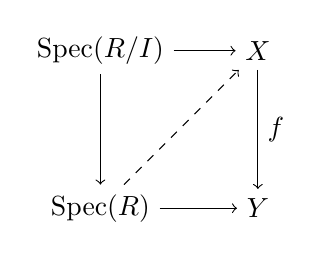
\begin{tikzpicture}
                \node (X) at (0, 1) {$X$};
                \node (Y) at (0, -1) {$Y$};
                \node (R) at (-2, -1) {$\mathrm{Spec}(R)$};
                \node (RI) at (-2, 1) {$\mathrm{Spec}(R/I)$};
                \draw[->] (X) -- node[right]{$f$} (Y);
                \draw[->] (RI) -- (X);
                \draw[->] (R) -- (Y);
                \draw[->] (RI) -- (R);
                \draw[->, dashed] (R) -- (X);
            \end{tikzpicture}
        \end{gather*}
        In other words, formally \'etale morphisms have the unique right lifting property with respect to infinitesimal thickenings. Analogously to the case of rings, the morphism $f$ is said to be \textbf{formally smooth} (resp.~\textbf{formally unramified}) if there is at least (resp.~at most) one lift.

        Since this definition does allow for some pathological examples, \'etale morphisms are defined as those morphisms that are formally \'etale and locally of finite presentation. (Likewise for smooth and unramified morphisms.)
    }

    \sremark{The term 'formally' should be interpreted in the sense of \textit{formal geometry} (see \labelref{chapter:hdg}). There, infinitesimal neighbourhoods of points (see \cref{hdg:infinitesimal_thickening}), used for defining the local geometry, are induced by nilpotent ideals. This is further exemplified by \cref{alggeom:tangent_cone_etale}.}

    \begin{property}[Equivalent conditions]
        The following conditions are equivalent for a scheme morphism $f:X\rightarrow Y$ locally of finite presentation:
        \begin{itemize}
            \item $f$ is \'etale,
            \item $f$ is flat and unramified,
            \item $f$ is flat and smooth, and
            \item $f$ is smooth and of relative dimension 0.
        \end{itemize}
        \todo{ADD Jacobian condition (see e.g.~\citet{mumford_red_1999})}
    \end{property}
    \begin{property}[Fibres]
        An \'etale morphism has discrete fibres.\footnote{This actually holds for all unramified morphisms.} In particular, if it is quasicompact, it has finite fibres.
    \end{property}

    \begin{remark}\label{alggeom:etale_remark}
        As a side note, the general definition of \'etale morphism is related to \cref{alggeom:etale_morphism_variety}. The completion of the local ring $\mathcal{O}_x$ is defined by the inverse limit over the filtration $\mathcal{O}_x/\mathfrak{m}_x\leftarrow\mathcal{O}_x/\mathfrak{m}_x^2\leftarrow\mathcal{O}_x/\mathfrak{m}_x^3\leftarrow\cdots$. Hence, a morphism $\widehat{\mathcal{O}}_x\rightarrow\widehat{\mathcal{O}}_y$ between completions is characterized by consecutive lifting problems, which are exactly the content of \cref{algebra:formally_etale}, since the ideals $\mathfrak{m}_x$ are clearly nilpotent in rings of the form $\mathcal{O}_x/\mathfrak{m}_x^k$ for any $k\in\mathbb{N}_0$.
    \end{remark}
    This is generalized to schemes as follows.
    \begin{property}\label{alggeom:etale_conditions}
        If $Y$ is locally Noetherian and $f:X\rightarrow Y$ is locally of finite presentation, \'etale morphisms can also be characterized in terms of completions. $f$ is \'etale if and only if the induced morphism on completions is formally \'etale in the adic topology.

        Moreover, if $\kappa(x)\cong f^\sharp\bigl(\kappa(x)\bigr)$, $f$ is \'etale if and only if the induced morphisms of completions are isomorphisms (as in the case of affine varieties over algebraically closed fields).
    \end{property}

    \newdef{Finite \'etale morphism}{\index{etale!morphism}
        A morphism of schemes $f:X\rightarrow Y$ for which there exists a covering $\{U_i\}_{i\in I}$ of $Y$ by affine sets $U_i\equiv\mathrm{Spec}(A_i)$ such that $f^{-1}(U_i)\cong\mathrm{Spec}(B_i)$ is a free, separable $A_i$-algebra $B_i$ for all $i\in I$.
    }
    \begin{remark}[Finite \'etale covering]\index{etale!covering}
        When a finite \'etale morphism $f:X\rightarrow Y$ exists, $X$ is sometimes called a \textbf{finite \'etale cover(ing)} of $Y$. The full subcategory of the slice category $\symbfsf{Sch}/_Y$ on finite \'etale coverings is often denoted by $\symbfsf{FEt}_X$.
    \end{remark}

    \newdef{\'Etale fundamental group}{\index{fundamental group!etale}
        Consider a connected scheme $X$. The (\'etale) fundamental group $\pi_1(X)$ is the unique (up to isomorphism) profinite group \ref{topology:profinite_group} such that $\symbfsf{FEt}_X$ is equivalent to the category $\symbfsf{Fin}\,\pi_1(X)\symbfsf{Set}$ of finite of $\pi_1(X)$-sets.
    }
    \begin{remark}
        Recall \cref{topology:equivalent_categories} for topological spaces. There, a stricter set of spaces was considered with the benefit that all $\pi_1(X)$-sets could be classified. By passing to profinite groups one can formulate a classification statement in the topological setting that is virtually identical to the above one.
    \end{remark}

    The following definition is analogous to \cref{topology:proper_function}.
    \newdef{Proper morphism}{\index{proper}\index{closed}
        A scheme morphism $f:X\rightarrow Y$ satisfying
        \begin{enumerate}
            \item $X$ is separated as a $Y$-scheme,
            \item $f$ is of finite type, and
            \item $f$ is \textbf{universally closed}, i.e.~the pullback along any scheme morphism is closed.
        \end{enumerate}
    }

\subsection{Subschemes}

    Since general schemes need not be reduced, the structure sheaf could have nilpotent sections. Consequently, restricting a structure sheaf $\mathcal{O}_X$ along a topological inclusion $Y\subseteq X$ is (generally) not possible, since nilpotent sections are not determined by their values at points.

    \newdef{Closed subscheme}{
        Let $(X,\mathcal{O}_X)$ be a scheme. A (closed) subscheme is defined by the following data:
        \begin{enumerate}
            \item A closed subset $Y\subseteq X$,
            \item A sheaf $\mathcal{O}_Y$ such that $(Y,\mathcal{O}_Y)$ is a scheme, and
            \item A surjection $\pi:\mathcal{O}_X\twoheadrightarrow\mathcal{O}_Y$, i.e.~a sheaf morphism whose maps on stalks are surjections.
        \end{enumerate}
    }

    \begin{property}[Ideal sheaf]\index{ideal!sheaf}
        If $\pi:X\rightarrow Y$ determines a closed subscheme, $\ker(\pi)$ is quasicoherent sheaf of ideals.
    \end{property}

    \begin{theorem}[Nullstellensatz]
        Closed subschemes of $X$ are equivalent to quasicoherent ideal sheaves on $X$.
    \end{theorem}

    \newdef{Closed immersion}{\index{immersion}
        A scheme morphism $f:X\rightarrow Y$ satisfying
        \begin{enumerate}
            \item (the underlying continuous function of) $f$ is injective,
            \item $f$ is closed, and
            \item $f^\sharp$ is a surjection.
        \end{enumerate}
    }

\subsection{Tangent space}

    \newdef{Tangent cone}{\index{tangent!cone}\index{initial!part}
        Consider an affine variety $X=V(I)$. The tangent cone to $X$ at the origin is defined as the zero locus of the `initial ideal' of $I$:
        \begin{gather}
            C_0X := V\bigl(\{f^{\text{in}}\bigm\vert f\in I\}\bigr)\,,
        \end{gather}
        where $f^{\text{in}}$ denotes the \textbf{initial part} of $f$, i.e.~the sum of the smallest degree monomials in $f$.
    }

    \newdef{Tangent space}{\index{tangent!space}
        Consider an affine variety $X$ and choose a point $x\in X$. By working in a suitable affine chart, one can assume that $x=0$. This implies that any polynomial $f\in I(X)$ has a vanishing constant term. The tangent space at $x$ is defined as follows:
        \begin{gather}
            T_xX := V\bigl(\{f^{[1]}\bigm\vert f\in I(X)\}\bigr)\,,
        \end{gather}
        where $f^{[1]}$ denotes the linear part of the polynomial $f$.
    }
    \begin{property}
        For $x=0$, one obtains that $I(0)=(x_1,\ldots,x_n)/I(X)$. Moreover, there exists a natural isomorphism
        \begin{gather}
            I(0)/I(0)^2\cong\hom_{\mathfrak{K}}(T_0X,\mathfrak{K})\,.
        \end{gather}
        The tangent space at $0$ can accordingly also be obtained as the dual of $I(0)/I(0)^2$.
    \end{property}

    It is not so hard to prove that this property can, in fact, easily be transported to arbitrary points $x\in X$ if one replaces the ideal $I(0)$ by the maximal ideal of the structure sheaf $\mathcal{O}_X$ at $x$. Therefore, one can give the following general definition.
    \newdef{Zariski tangent space}{\index{Zariski!tangent space}\label{alggeom:cotangent_space}
        Consider a scheme $X$ with structure sheaf $\mathcal{O}_X$. At every point $x\in X$, the stalk $\mathcal{O}_x$ is a local ring and, hence, has a maximal ideal $\mathfrak{m}_x$. The quotient $\mathfrak{m}_x/\mathfrak{m}_x^2$ is a vector space over the residue field $\mathcal{O}_x/\mathfrak{m}_x$. It is called the Zariski cotangent space at $x\in X$ and its algebraic dual is called the Zariski tangent space at $x\in X$.
    }

    \begin{property}[Finite-dimensionality]
        If $x\in X$ is closed, $T_xX\cong T^*_xX$.
    \end{property}

    \newdef{Regular scheme}{\index{regular!scheme}
        A (Noetherian) scheme is said to be regular or \textbf{nonsingular} if the local dimension at any point is equal to the dimension of the Zariski tangent space at that point. Equivalently, an affine variety is smooth if at every point the tangent space is isomorphic to the tangent cone.
    }

    \newadef{Tangent cone: Schemes}{\index{tangent!cone}
        Assume that $X$ is a Noetherian scheme. The tangent cone $C_xX$ is given by the spectrum of the graded ring $\mathrm{Gr}(\mathcal{O}_x)=\bigoplus_{k\in\mathbb{N}}\mathfrak{m}_x^k/\mathfrak{m}_x^{k+1}$. If $X$ is regular, the tangent cone coincides with the Zariski tangent space.
    }

    \begin{remark}[Inverse function theorem]\index{inverse function theorem}
        In the smooth setting (see \labelref{chapter:manifolds} and onwards), the inverse function theorem states that a tuple of functions forms a local coordinate system at a point if their \textit{differentials} generate the \textit{cotangent space} at that point.

        Here, the ideal $\mathfrak{m}_x$ consists of the functions vanishing at $x\in X$ and the cotangent space is given by $\mathfrak{m}_x/\mathfrak{m}_x^2$. By Nakayama's lemma~\ref{algebra:nakayama}, a tuple of elements represent `coordinate functions', i.e.~generate $\mathfrak{m}_x$, if their `differential', i.e.~their residues in the Zariski cotangent space, generate the cotangent space.

        For schemes, the inverse function theorem becomes the following. If a point $x\in X$ is regular, there exists a neighbourhood which is an (affine) variety.
    \end{remark}

    Recall \cref{alggeom:etale_morphism_variety} of \'etale morphisms of affine varieties (over algebraically closed fields) and \cref{alggeom:etale_conditions} for schemes. The following property relates these to the infinitesimal thickening point-of-view.
    \begin{property}\label{alggeom:tangent_cone_etale}
        A morphism $f:X\rightarrow Y$ of finite type of Noetherian schemes is \'etale if and only if it induces an isomorphism on tangent cones.
    \end{property}

    \begin{property}
        If $X$ is a scheme over a field $\mathfrak{K}$ and $x\in X$ is closed, the tangent space at $x$ admits an `alternative' description:
        \begin{gather}
            T_xX \cong \symbfsf{Sch}_{\mathfrak{K}}\left(\spec(\mathfrak{K}[\varepsilon]/\varepsilon^2),X\right)\,.
        \end{gather}
    \end{property}

    \begin{property}[Dimension]
        If $X$ is (locally) Noetherian, then
        \begin{gather}
            \dim(T_xX)\geq\dim(X)\,.
        \end{gather}
    \end{property}

\subsection{Algebraic de Rham complex}\index{de Rham!complex}

    For this section, the notion of \textit{K\"ahler differential} is used (see \cref{nca:kahler_differential}). For an affine scheme $X\equiv\mathrm{Spec}(R)$, where $R$ is finitely generated over $\mathfrak{K}$, let $\Omega_{X/\mathfrak{K}}$ denote the algebra of K\"ahler differentials. If $X$ is smooth, $\Omega_{X/\mathfrak{K}}$ will be locally free of rank $\dim(X)$.

    In a relative setting, one obtains the relative K\"ahler differentials $\Omega_{R/S}$ induced by the multiplication $\mu:R\otimes_SR\rightarrow R$. Globalizing leads to the diagonal morphism $\Delta:X\rightarrow X\times_YX$ which gives a closed subscheme $\Delta(X)$. By the Nullstellensatz, every closed subscheme is induced by a quasicoherent sheaf of ideals $\mathcal{I}$. Repeating the construction of K\"ahler differentials, one can construct the (quasicoherent) sheaf $\mathcal{I}/\mathcal{I}^2$.

    \newdef{Conormal sheaf}{\index{conormal!sheaf}
        Let $f:X\rightarrow Y$ be a scheme morphism. The conormal sheaf $\Omega_{X/Y}$ is defined as the pullback $\Delta^*(\mathcal{I}/\mathcal{I}^2)$.
    }

    The differential $\dr$ on $\Omega_{X/Y}$ can be defined by pullback as well:
    \begin{gather}
        \dr:\mathcal{O}_X\rightarrow\Omega_{X/Y}:f\mapsto\Delta^*(\pi_2^*f-\pi_1^*f)\,,
    \end{gather}
    where $\pi_1,\pi_2:X\times_YX\rightarrow X$ are the canonical projections. This derivation is $\mathcal{O}_Y$-linear.

    \begin{property}
        If $X\rightarrow Y$ is locally of finite type and $X$ is locally Noetherian, $\Omega_{X/Y}$ is coherent.
    \end{property}

    \begin{property}[Pullback stability]
        Consider the pullback $X':=Y'\otimes YX$. There exists an isomorphism
        \begin{gather}
            \pi_X^*\Omega_{X/Y}\cong\Omega_{X'/Y'}\,. 
        \end{gather}
    \end{property}
    \begin{result}
        The sheaf of differentials on a fibre coincides with the fibre of the sheaf of differentials. 
    \end{result}

    Recall \cref{alggeom:cotangent_space}. This space can be obtained by taking fibres.
    \begin{property}[Cotangent space]\index{Zariski!tangent space}
        The cotangent space at a point $x\in X$ of a scheme $X\rightarrow Y$ is equal to
        \begin{gather}
            T_x^*X = \Omega_{X/Y,x}\otimes_{\mathcal{O}_{X,x}}\kappa(x)\,.
        \end{gather}
    \end{property}

    \todo{COMPLETE}

\section{\difficult{Topos theory}}

    This section also uses the content of \labelref{chapter:topos}.

    \newdef{Zariski topology}{\index{Zariski!topology}
        The Zariski topology on the category of schemes is generated by sets $\{f_i:U_i\rightarrow X\}_{i\in I}$ of open immersions such that $X=\bigcup_{i\in I}f_i(U_i)$ in the set-theoretic sense. This latter condition is often called \textbf{joint surjectivity}. This gives the \textbf{big Zariski site} on an a scheme $X$. The \textbf{small Zariski site} of a scheme $X$ is the subsite of $\symbfsf{Sch}_{/X}$ on the open immersions.
    }
    \begin{remark}[Size issues]
        There are some size issues with the category of schemes, it being a big category. The result is that in general there exists no sheafification functor, i.e.~no general construction of the category of sheaves and, hence, this category can only be turned into a site, not a (Grothendieck) topos.\footnote{One can actually also work with large sites to obtain topoi as long as they contain a \textit{small topologically generating set} or, even more general, satisfy the \textit{WISC axiom}.} In the case of \textit{topological} or \textit{smooth manifolds}, this problem is often ignored since one has a (small) dense subsite and no issues arise. For schemes, however, the situation is different. For example, the fpqc topology (to be introduced below) does not admit a sheafification functor. Two solutions exists in such a context, either one works within a suitable universe or one only considers a single (pre)sheaf at a time.
    \end{remark}

    \begin{property}
        The Zariski site is subcanonical.
    \end{property}

    The following topology is finer than the Zariski topology.\footnote{There exists another topology in between the Zariski and \'etale topologies, the \textit{Nisnevich topology}, but this is of no interest here.}
    \newdef{\'Etale cover}{\index{cover!\'etale}\index{site!\'etale}
        An \'etale cover of a scheme $X$ is a jointly surjective family of \'etale morphisms that are locally of finite type\footnote{For $X$ locally Noetherian, this additional condition is superfluous.}. The \textbf{big \'etale site} $\symbfsf{Sch}_{/X,\text{\'et}}$ is the slice category of $X$ equipped with the coverage (see \cref{topos:coverage}) of \'etale covers. The \textbf{small \'etale site} is the subsite on \'etale morphisms.
    }

    \begin{property}
        A presheaf satisfies descent with respect to the \'etale topology if and only if it satisfies descent with respect to the following covers:
        \begin{itemize}
            \item Zariski covers, and
            \item (single) faithully flat morphisms of affine schemes.
        \end{itemize}
    \end{property}

    \newdef{Flat topologies}{\index{flat!topology}
        The finest topologies on the category of schemes (or slices thereof) are given by considering flat morphisms. The two most widely used flat topologies are the `fppf-' and `fpqc-topologies'. The \textbf{fppf-topology} (for \textit{fid\`element plat de presentation finie}) is generated by jointly surjective families of flat morphisms that are locally of finite presentation. The \textbf{fpqc-topology} (for \textit{fid\`element plat et quasi-compacte}) is generated by jointly surjective families of flat and quasicompact morphisms.
    }
    \begin{remark}
        As defined above, the fpqc-topology is technically not comparable to the Zariski topology, since open immersions need not be quasicompact (unless one restricts to Noetherian schemes). A solution introduced by \indexauthor{Vistoli} and \indexauthor{Kleiman} is to replace quasicompactness by the following seemingly similar definition: There exists an open affine cover $\{U_i\}_{i\in I}$ of $X$ such that each $U_i$ is the image of a compact open subscheme. (If one drops the modifier `locally' in the definition of the fppf-topology, a similar problem arises.)
    \end{remark}
    \begin{remark}[Standard covers]
        An equivalent approach to the definition of flat topologies is by first defining `standard' fppf or fpqc covers on affine schemes. These are similar to the flat covers defined above, but where the families are finite and the codomains affine. The covers of general schemes are then generated by base change.
    \end{remark}

    By interpreting objects in the big topos (over a scheme) as generalized spaces in the sense of \labelref{chapter:hdg}, the following definition is obtained.
    \newdef{Algebraic space}{\index{algebraic!space}\index{atlas}\label{alggeom:algebraic_space}
        An object $X\in\symbfsf{Sh}(\symbfsf{Sch}_{\text{fppf}})$ satisfying
        \begin{enumerate}
            \item The diagonal morphism $X\rightarrow X\times X$ is \textit{representable} (see \cref{topos:representable_diagonal}).
            \item There exists a scheme morphism $Y\rightarrow X$ that is surjective and \'etale. This is sometimes called an \textbf{atlas}.
        \end{enumerate}
        Requiring representability of the diagonal can be argued as follows. The fibre product can be seen as a generalized notion of intersection, so representability means that the intersection of any two schemes is again a scheme. Moreover, representability of the diagonal also implies representability of the atlas.
    }

    \newdef{Local property}{\index{local!property}\label{alggeom:local_property}
        Consider some property of scheme morphisms $P$, e.g.~\'etale or smoothness. Relative to some topology on $\symbfsf{Sch}$, the property $P$ is said to be \textbf{local on the source} if for every cover $\{X_i\rightarrow X\}_{i\in I}$ and every morphism $f:X\rightarrow Y$ the following holds:
        \begin{gather}
            f\text{ satisfies }P\iff\forall i\in I:X_i\rightarrow Y\text{ satisfies }P\,.
        \end{gather}
        Analogously, the property $P$ is said to be \textbf{local on the base} or \textbf{local on the target} if for every cover $\{Y_i\rightarrow Y\}_{i\in I}$ and every morphism $f:X\rightarrow Y$ the following holds:
        \begin{gather}
            f\text{ satisfies }P\iff\forall i\in I:Y_i\times_YX\rightarrow Y_i\text{ satisfies }P\,.
        \end{gather}
    }

    Inspired by locality, one can generalize many properties of scheme morphisms to morphisms of algebraic spaces.
    \newdef{Property of algebraic spaces}{
        Consider a representable morphism of algebraic spaces $F:X\rightarrow Y$. If $P$ is a property of scheme morphisms satisfying:
        \begin{enumerate}
            \item it is preserved under base change, and
            \item it is fppf-local on the target,
        \end{enumerate}
        then $f$ is said to have the property $P$ if for all $T\in\ob{Sch}$ and all $G:h_T\rightarrow Y$ the morphism $S_G\rightarrow T$ has property $P$, where $S_G\in\ob{Sch}$ is a representing object of $G$, i.e.~$h_{S_G}\cong h_T\times_YF$.
    }
    \newdef{\'Etale morphism}{\index{etale!morphism}
        A morphism $F:X\rightarrow Y$ of algebraic spaces such that for every \'etale morphism $G:h_S\rightarrow X$ the composition $f\circ g$ is also \'etale.\footnote{In a similar vein, one can define smooth morphisms of algebraic spaces.}
    }

\section{Algebraic groups \& Galois theory}\index{Galois!theory}

    For some background on Galois theory, see \labelref{section:galois_extensions}.

\subsection{Weil restriction}

    Consider a $\mathfrak{K}$-variety $X\rightarrow\spec(\mathfrak{K})$ such that $X$ is characterized by polynomials with coefficients in a subfield $\mathfrak{K}_0$. In this case, one has
    \begin{gather}
        X\cong\spec\left(\mathfrak{K}_0[x_1,\ldots,x_n]/I_0\right)\times_{\spec(\mathfrak{K}_0)}\spec(K)\,.
    \end{gather}
    Such a variety $X$ is said to be \textbf{defined over $\mathfrak{K}_0$}. (This also works for schemes.)

    A related notion is the following.
    \newdef{Weil restriction}{\index{Weil!restriction}\index{restriction!of scalars}
        Consider an $\mathfrak{L}$-scheme $X$ together with a field extension $\mathfrak{L}/\mathfrak{K}$. One can obtain a $\mathfrak{K}$-scheme by \textbf{restriction of scalars}\footnote{This adjunction is inherited from an adjunction on rings.}:
        \begin{gather}
            \symbfsf{Sch}_{\mathfrak{K}}\left(S,\mathrm{Res}_{\mathfrak{L}/\mathfrak{K}}X\right) := \symbfsf{Sch}_{\mathfrak{L}}\left(S\times_{\spec(\mathfrak{K})}\mathfrak{L},X\right)\,.
        \end{gather}
    }
    
    Now, consider a field extension $\mathfrak{L}/\mathfrak{K}$ and a $\mathfrak{K}$-scheme $X$. From this, one can construct an $\mathfrak{L}$-scheme as above by base change:
    \begin{gather}
        \widetilde{X} := X\times_{\mathfrak{K}}\spec(\mathfrak{L})\,.
    \end{gather}
    Every automorphism $\sigma\in\Aut(\mathfrak{K}/\mathfrak{L})$ induces an automorphism on $\widetilde{X}$. Note that, on the unique stalk of the affine factor, $f^*=\sigma^{-1}$ by contravariance.

    \begin{property}[Galois action]
        If $\mathfrak{L}=\overline{\mathfrak{K}}$, the fibre $\pi^{-1}(x)$, with respect to the projection $\pi:\widetilde{X}\rightarrow X$, is a finite orbit of the $\Aut(\overline{\mathfrak{K}}/\mathfrak{K})$-action. In fact,
        \begin{gather}
            X \cong \widetilde{X}/\Aut(\overline{\mathfrak{K}}/\mathfrak{K})
        \end{gather}
        as topological spaces.
    \end{property}
    \begin{remark}[Ambient category]
        As schemes, the quotient above is not isomorphic to $X$. One needs more, such as $\mathfrak{K}$ being perfect (\cref{algebra:perfect_field}), hence working with Galois extensions, and $X$ being reduced.
    \end{remark}

    \begin{remark}[Galois descent]\index{Galois!descent}\index{form}
        Although only a small introduction to the topic was presented here, a vast amount of work exists on recovering subschemes from Galois actions (and beyond). The keywords here are `\textit{forms}' and `\textit{Galois descent}' (see e.g.~\citet{milne_descent_2024}).
    \end{remark}

\subsection{Galois theory}

    \begin{property}[Fixed points]
        When $\mathfrak{K}$ is perfect, the fixed points of $\mathrm{Gal}(\mathfrak{L}/\mathfrak{K})$ correspond to the $\mathfrak{K}$-rational points of the form $\pi(x)$ for $x\in\widetilde{X}$.
    \end{property}

    \newdef{Absolute Galois group}{
        The Galois group $\mathrm{Gal}(\mathfrak{K}_S/\mathfrak{K})$ of the separable closure (\cref{algebra:separable_closure}) of $\mathfrak{K}$.
    }

    The following property relates Galois theory to algebraic geometry.
    \begin{property}[Grothendieck's Galois theory]\index{Grothendieck}
        Consider a field $\mathfrak{K}$ with separable closure $\mathfrak{K}_S$.
        \begin{gather}
            \mathrm{Gal}(\mathfrak{K}_S/\mathfrak{K})\cong\pi_1\bigl(\mathrm{Spec}(\mathfrak{K})\bigr)\,,
        \end{gather}
        where $\pi_1$ is the \'etale fundamental group (the fundamental group at the topological level would not carry a lot of information since $\mathrm{Spec}(\mathfrak{K})$ is a one-point space).
    \end{property}

    

    \newdef{Group scheme}{\index{group!scheme}
        A group object in $\symbfsf{Sch}$.
    }
    \begin{example}[Additive group]\index{group!additive}
        The additive group $\mathbb{G}_a$ (over some field $\mathfrak{K}$) has as underlying object the affine line $\spec(\mathfrak{K}[x])$ and as operations:
        \begin{enumerate}
            \item\textbf{Addition}: Dual of the ring morphism $\mathfrak{K}[x]\rightarrow \mathfrak{K}[x_1]\otimes \mathfrak{K}[x_2]:x\mapsto x_1+x_2$.
            \item\textbf{Unit}: Dual of $\mathfrak{K}[x]\rightarrow\mathbb{Z}:x\mapsto0$.
            \item\textbf{Inversion}: Dual of $\mathfrak{K}[x]\rightarrow \mathfrak{K}[x]:x\mapsto-x$.
        \end{enumerate}
        Equivalently, it is the $\symbfsf{Ab}$-valued functor that sends a scheme to the Abelian group of global sections of its structure sheaf.
    \end{example}

    \newdef{Linear algebraic group}{\index{group!algebraic}
        A subgroup of $\GL(n,\mathfrak{K})$ defined by a (finite) set of polynomials in the matrix coefficients.
    }
    \begin{property}
        From the definition, it is immediately clear that intersections of algebraic groups are again algebraic.
    \end{property}

    \newdef{Abelian variety}{\index{variety!Abelian}\label{alggeom:abelian_variety}
        A smooth, projective and algebraic group.
    }
    \begin{theorem}[Mordell--Weil]
        For an Abelian variety $X$ over a number field $\mathfrak{K}$ (\cref{algebra:number_field}), the set of rational points $X(\mathfrak{K})$ (\cref{alggeom:rational_point_scheme}) is a finitely generated Abelian group.
    \end{theorem}

\section{Tropical geometry}\index{tropical geometry}

    The following definition generalizes \cref{group:ring}.
    \newdef{Rig}{\index{rig}
        Let $R$ be a set equipped with two binary operations $+,\cdot$ (called\footnote{This might become confusing when looking at the examples below.} \textbf{addition} and \textbf{multiplication}). $(R,+,\cdot)$ is a rig if it satisfies the following axioms:
        \begin{enumerate}
            \item $(R,+)$ is a commutative monoid.
            \item $(R,\cdot)$ is a monoid.
            \item Multiplication is distributive with respect to addition.
        \end{enumerate}
    }
    \begin{remark}
        Whereas a ring is a group object in $\symbfsf{CRing}$, a rig is a group object in $\symbfsf{CMonoid}$. (The monoidal structures on these categories should not be taken to be the Cartesian ones for this result).
    \end{remark}

    \begin{example}[Tropical rig]
        Consider the set $T:=\mathbb{R}\cup\{+\infty\}$. This set becomes a rig when equipped with the following operations:
        \begin{enumerate}
            \item\textbf{Addition}: $x\oplus y=\min(x,y)$.
            \item\textbf{Multiplication}: $x\cdot y=x+y$.
        \end{enumerate}
    \end{example}

    \newdef{Tropicalization}{\index{tropicalization}\index{Puiseux series}
        In ordinary algebraic geometry, one considers polynomials over $\mathbb{R}$ as the basic building blocks. These also give rise to polynomials over $T$. To every polynomial
        \begin{gather}
            f = a+\sum_{i=1}^k\lambda_ix^{n_i}_i
        \end{gather}
        with $a\in\mathbb{Z}$, one assigns its tropicalization
        \begin{gather}
            \mathrm{trop}(f) := \min(0,n_1x_1,\ldots,n_kx_k)\,.
        \end{gather}
        Note that the tropicalization of any polynomial is a piecewise linear function.

        A more formal definition goes as follows. Let $\mathfrak{K}_P$ be the ring of \textbf{Puiseux series}, i.e.~of elements of the form
        \begin{gather}
            a = \sum_{i=k}^{+\infty}\lambda_ix^{i/n}
        \end{gather}
        for some $k,n\in\mathbb{N}$. These generalize Laurent series (\cref{complex:laurent_series}) to fractional exponents in that $\mathfrak{K}_P=\bigcup_{i\in\mathbb{N}_0}\mathbb{C}((x^{1/i}))$. Then, consider the valuation (\cref{algebra:valuation})
        \begin{gather}
            \mathrm{val}:\mathfrak{K}_P\rightarrow\mathbb{R}:a\mapsto\min\{i/k\mid\lambda_i\neq0\}\,.
        \end{gather}
        The tropicalization of
        \begin{gather}
            f = \sum_{u\in\mathbb{N}^n}\lambda_ux^u
        \end{gather}
        with $n\in\mathbb{N}$ is given by
        \begin{gather}
            \mathrm{trop}(f) := \min_{u\in\mathbb{N}^n,\lambda_u\neq 0}\bigl(\mathrm{val}(\lambda_u)+\sum_{i=1}^nu_ix_i\bigr)\,.
        \end{gather}
    }

    \todo{COMPLETE (link with mirror symmetry \citep{gross_tropical_2011})}